\documentclass[11pt]{article}
\usepackage[T1]{fontenc}
\usepackage[utf8]{inputenc}
\usepackage{lmodern}
\usepackage{microtype}
\usepackage[margin=1in]{geometry}
\usepackage{setspace}
\usepackage{amsmath,amssymb,amsthm}
\usepackage{mathtools}
\usepackage{bm}
\usepackage{graphicx}
\usepackage{booktabs}
\usepackage{tabularx}
\usepackage{array}
\usepackage{enumitem}
\usepackage{xcolor}
\usepackage{caption}
\usepackage{subcaption}
\usepackage{tikz}
\usetikzlibrary{arrows.meta,positioning,calc,decorations.pathreplacing}
\usepackage[authoryear,round]{natbib}
\usepackage{xurl}
\usepackage[hidelinks]{hyperref}
\usepackage{cleveref}

\theoremstyle{plain}
\newtheorem{proposition}{Proposition}
\newtheorem{lemma}{Lemma}
\newtheorem{corollary}{Corollary}
\theoremstyle{definition}
\newtheorem{assumption}{Assumption}
\newtheorem{definition}{Definition}
\theoremstyle{remark}
\newtheorem{remark}{Remark}

\crefname{proposition}{Proposition}{Propositions}
\crefname{lemma}{Lemma}{Lemmas}
\crefname{corollary}{Corollary}{Corollaries}
\crefname{assumption}{Assumption}{Assumptions}
\crefname{remark}{Remark}{Remarks}
\crefname{definition}{Definition}{Definitions}
\crefname{section}{Section}{Sections}
\crefname{subsection}{Section}{Sections}
\crefname{appendix}{Appendix}{Appendices}
\crefname{subappendix}{Appendix}{Appendices}
\crefname{table}{Table}{Tables}
\crefname{figure}{Figure}{Figures}
\crefname{equation}{equation}{equations}
\creflabelformat{equation}{(#2#1#3)}


\newcommand{\pos}[1]{\left[#1\right]^{+}}
\setlist{itemsep=2pt,topsep=4pt}

\onehalfspacing

\title{Europe's ASML Card in Three Numbers: A Minimal Model}
\author{Matt DiGiuseppe\thanks{Working note, \today. Companion to \emph{Owning the Chokepoint: ASML, Alliance Dependence, and the Limits of Europe's Leverage over Washington} (working draft, 29 October 2026). Almost all of this note was written by Claude, an AI system made by Anthropic, working in Claude Code. Matt DiGiuseppe's contribution was the research question, the instructions and the reading material. Every numbered result is a special case of a result proved in the full paper (with China's offer fixed rather than bid), and each was checked by brute-force computation (\texttt{code/checks/minimal\_model\_check.py}).} \and Claude (Anthropic)}
\date{\today}

\begin{document}
\maketitle

\begin{abstract}
\noindent The full paper explains how much bargaining power Europe draws from ASML, the only maker of the machines that print the most advanced AI chips, with a model that has many moving parts. This note keeps three numbers: what China's offer is really worth to Europe, what Washington would really cut off if Europe switched sides, and what Washington would lose if it did. Europe's price is set by its walk-away value, the first number minus the second. Washington's need for ASML, the reason \emph{Europe 2031} calls it Europe's last card, does not raise the price. When the walk-away value is negative, a Washington whose threats stick can extract concessions up to the gap, its squeeze room, and every demand it makes draws on that single budget. Washington's need raises Europe's price only if stalled talks risk a realignment neither side chose, Europe sometimes names the terms, and Washington cannot use threats to take the gain back. A halt to servicing adds to the price only if Europe can tie its own hands. When Europe's walk-away value is set to turn positive and Washington has nothing better to spend its squeeze room on, Washington has a reason to demand control of ASML while it still can, provided the squeeze room exceeds what handing over control would cost Europe.
\end{abstract}

\section{The question}

ASML, a Dutch firm, is the only company that builds extreme ultraviolet lithography machines, and the most advanced AI chips cannot be made without them. A scenario published in June 2026, \emph{Europe 2031}, calls ASML ``the only card Europe still holds'' \citep{juijn2026europe}. Yet since 2019 the Netherlands has gone along with Washington's demands to restrict sales to China and has been paid nothing for it \citep{nltimes2020pressured, govnl2023controls}. What it received in December 2024, an exemption from new US rules on foreign-made chip tools \citep{bis2024fdpr}, is a status Washington can take back by changing a rule. If Washington needs ASML so badly, why has Europe got so little for it?

Our answer is that Europe is paid for what it could get by switching sides, net of what it would lose, and on our reading that number has been negative since 2019.

\section{Three numbers and one rule}

Three numbers describe the bargain, all in one currency: a payment worth a unit to Europe costs Washington a unit.

\begin{description}[leftmargin=1.2em, labelindent=0em]
\item[China's offer, $c\ge 0$.] What China would really give Europe for switching sides and supplying it. Europe discounts Chinese promises it doubts, and China will not pay for what US legal reach over the American parts and staff ASML relies on would block anyway.
\item[Washington's penalty, $k\ge 0$.] What Washington would really cut off if Europe switched: the American parts and staff ASML relies on, access to frontier AI, and the part of its security support it would withdraw from a disloyal ally. Support Washington would give Europe anyway, for its own reasons, is not part of $k$, however large that support is.
\item[Washington's need, $V>0$.] What Washington would lose if Europe switched and China got the tools.
\end{description}

\noindent Europe's \emph{walk-away value}, $c-k$, is how much better off Europe would be by switching, all things counted. When it is negative, its size $k-c$ is Washington's \emph{squeeze room}.

\paragraph{The rule.} Washington names a deal. It can offer Europe a payment, or demand concessions such as tighter controls on sales to China, and it can back the deal with a threat to cut off $k$ if Europe refuses. Europe accepts or refuses. If it refuses and the threat is carried out, Europe decides whether to switch sides. We say the threat \emph{sticks} if Washington has bound itself to carry it out after a refusal, for instance by making it public at a cost it cannot walk back. A threat that does not stick leaves Washington to decide afresh, after a refusal, whether cutting Europe off is worth it.

Washington names the deal because the status quo already gives it what it wants: Europe stays aligned and ASML's machines keep flowing to American and allied chip plants. If talks stall, Washington loses nothing, so it can turn down any European demand and come back with its own offer. Giving Washington the first move is a shortcut for that fact. \Cref{sec:need} lets Europe name the terms some of the time.

\emph{Carrying out the threat frees Europe.} Once Washington has cut off $k$, Europe has nothing more to lose by switching, and switching gains it $c$. A Europe that refuses can therefore always end up at $c-k$, and no threat can push it lower. A threat to cut off $k$ takes at most $k-c$, not $k$.

\section{What Europe gets}\label{sec:gets}

\begin{proposition}[Price and squeeze]\label{min:price}
Europe always gets at least its walk-away value $c-k$. If Washington's threat sticks, Washington offers exactly $c-k$: it pays Europe $c-k$ when China's offer exceeds Washington's penalty, and takes concessions worth $k-c$ when it does not. If the threat does not stick and $c>0$, Washington pays $c-k$ when that is positive and nothing otherwise. Either way, Washington keeps Europe if $c-k<V$ and lets it go if $c-k>V$.
\end{proposition}

Europe's price is set by its walk-away value. Washington's need, $V$, which \emph{Europe 2031} counts on, decides only whether Washington would rather pay or let Europe go. It does not raise the price. Threats matter only when the walk-away value is negative. When it is positive, Washington has to pay it, threats or no threats. When it is negative, a Washington whose threats do not stick pays nothing and gets nothing. A Washington whose threats stick takes concessions worth the whole squeeze room. \Cref{fig:minimal} shows both cases.

On our reading the Dutch record since 2019 fits a negative walk-away value: Washington has paid nothing. US legal reach over the American parts and staff ASML relies on does much of the work, by shrinking what China could offer and adding to what Washington could cut off.

\begin{figure}[t]
\centering
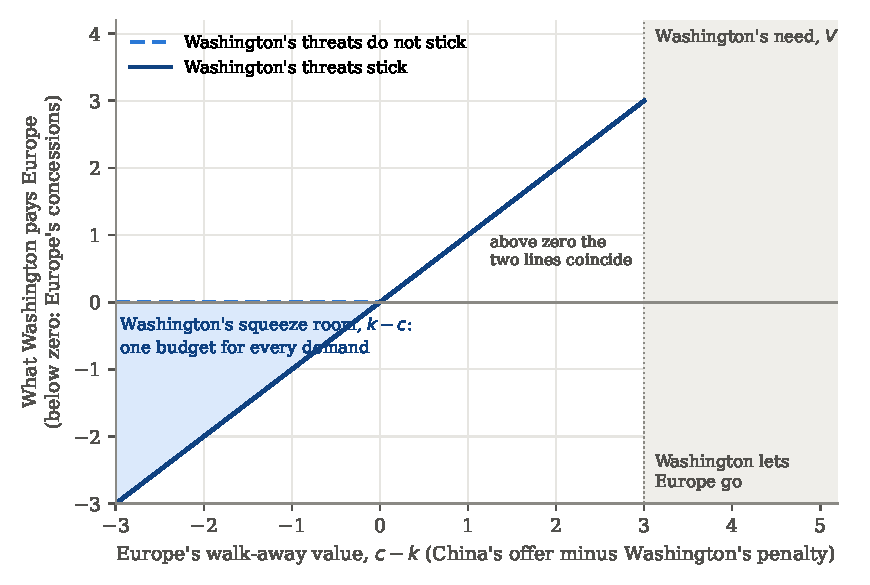
\includegraphics[width=\textwidth]{fig_minimal.pdf}
\caption{What Europe gets for ASML. The lines show what Washington pays Europe at each walk-away value (China's offer minus Washington's penalty). Above zero, payment equals the walk-away value, whatever Washington's need. Washington's need $V$ sets only where the lines stop and Washington lets Europe go; more need ($V'$) moves that point to the right without lifting the line. Below zero, a Washington whose threats stick takes concessions equal to the squeeze room (shaded), and every demand draws on it; one whose threats do not stick takes nothing. Illustrative units.}
\label{fig:minimal}
\end{figure}

\begin{proposition}[One budget]\label{min:budget}
However Washington combines its demands and threats, it cannot take more than $k-c$ from Europe in total.
\end{proposition}

Every American demand draws on the same squeeze room: export controls, limits on servicing machines already in Chinese plants, tariff cuts, arms purchases, defence spending. A concession won on one issue leaves less to win on the others. Splitting its threats across issues does not help Washington, because carrying out one raises Europe's walk-away value by the amount withdrawn, and the remaining threats bite less. Washington is sure of the full budget only if it makes all its demands at once. Piecemeal demands can get less, because a Europe that expects more demands to follow its concessions has less reason to make them \citep{pauly2024damned}.

The budget would make sense of a pattern in the record. The Netherlands gave way on controls over the sale of new machines. Yet as of mid-2026 ASML was still allowed to service machines it had installed in Chinese plants \citep{zakaria2026match}, and the Dutch cabinet objected when a bill in Congress, the MATCH Act, proposed reaching into allied countries to stop that \citep{baumgartner2026match, tk2026match}. If Washington had won the sales controls by threatening to withdraw support, this would be a government rationing concessions within a fixed budget. We have found no such threat behind the Dutch sales controls. Our reading is that US legal reach blocked those sales directly, which uses up no budget because Washington never has to carry out a threat, and that Washington came to servicing late because until 2026 it had no such reach over ASML's staff in China.

\section{When being needed pays}\label{sec:need}

\Cref{sec:gets} assumed that stalled talks cost nobody anything. Suppose instead that stalled talks cost Washington $X$ and Europe $Y$ for as long as they last, and that Europe names the terms a share $\beta$ of the time (Europe's say). Then Europe gets the larger of $c-k$ and
\[
\beta X-(1-\beta)Y .
\]
In words: Europe's say times what stalling costs Washington, less Washington's say times what stalling costs Europe.

Two things make stalled talks costly. Talks might collapse into a realignment that neither side chose, which costs Washington $V$ and, when Europe's walk-away value is negative, costs Europe its squeeze room, $k-c$. This is how Washington's need can enter the price. Or Europe might stop servicing the machines in American chip plants. While it lasts, the stoppage costs those plants $x$, the value of the servicing Washington cannot force ASML's American staff to keep doing, and costs Europe $y$, its own lost sales plus Washington's retaliation. Washington's cost $X$ blends the two: it is close to $V$ when collapse is likely and close to $x$ when it is not. Europe's cost $Y$ blends $k-c$ and $y$ the same way. The appendix gives the weights.

Being needed pays only under three conditions, the last of which concerns only a stoppage. First, Europe must have a say: if Washington always names the terms ($\beta=0$), Europe's power to hurt is worth nothing. Second, Washington must lack threats that stick and are large enough to push Europe back to its walk-away value. For the risk of collapse, the full paper shows that such threats take the gain back. We expect the same for a stoppage but have not proved it. Third, a stoppage counts only if Europe sets it before offers are made and cannot lift it after rejecting one. A stoppage Europe could lift after rejecting an offer is never used, at least in the equilibria the full paper studies: Europe would lift it at once to save its own costs, so Washington ignores it. The European Union's tools are built the other way. They let Brussels suspend countermeasures at once but escalate only slowly. Twice in 2025 the Union adopted countermeasures against Washington and then suspended them as soon as Washington moved \citep{commission2025suspension786, commission2025suspension1727}.

\section{When Washington wants control}\label{sec:control-min}

Washington's squeeze room lasts only while Europe's walk-away value stays negative. Rearmament, European computing capacity or a better Chinese offer would raise Europe's walk-away value and shrink the squeeze room.

\begin{proposition}[Control]\label{min:control}
Suppose Europe's walk-away value is negative today and will be positive tomorrow, Washington's threat sticks, and Washington has no other demand it values enough to spend today's squeeze room on. Then Washington demands control of ASML today, and Europe accepts, if and only if today's squeeze room, $k-c$, exceeds $s$, the political cost to Europe of handing over control.
\end{proposition}

Once Washington controls ASML, Europe has nothing left to sell China, so Washington never has to pay the positive walk-away value Europe will have tomorrow. Washington spends today's squeeze room to buy that. The handover costs Europe sovereignty and saves Washington only payments, so it destroys value. Like a preventive war, it is a costly move the stronger side makes now because its advantage is about to shrink. This is the logic of the ultimatum in \emph{Europe 2031}, in which Washington proposes folding ASML into a joint company it controls. If Washington could instead cash today's squeeze room in concessions worth as much to it as they cost Europe, it would take those and never bother with control.

\section{Where Washington's penalty comes from}

\Cref{min:price} takes the penalty $k$ as given. In fact it is partly Washington's choice: Washington decides how much of its security support to tie to Europe's loyalty, and tying support to loyalty costs it trust with every ally. A Washington that wants nothing beyond alignment ties at most enough support to bring Europe's walk-away value down to zero, and stops short if the lost trust becomes too costly first. It goes further only to create squeeze room it plans to spend. While the lost trust is cheap at the margin, Washington answers a stronger Chinese offer by tying more of its security support to Europe's loyalty, just enough to bring the walk-away value back to zero, and pays nothing. Once the lost trust is costly, it pays.

\section{What this note leaves out}

In the full paper, China puts a price on particular European concessions, as it did in the 2025 dispute over the chipmaker Nexperia \citep{taylorwessing2025nexperia, gerechtshof2025nexperia}, and that limits which concessions Washington can win. Europe does not decide as one: the Dutch government licenses sales to China, while any move against Washington needs the European Union. Each of Washington's threats sticks or does not stick on its own, and Washington may be unable to make some of them stick. Europe's own reluctance to arm a rival that backs Russia's war also lowers its walk-away value, but Washington cannot withdraw that reluctance, so the squeeze room can never exceed $k$. Washington's need also helps Europe indirectly, by making China bid more and by making Washington reluctant to punish a firm its own chip plants depend on.

On our reading of the record, US legal reach over the American parts and staff ASML relies on, which both shrinks China's offer and adds to Washington's penalty, can by itself keep Europe's walk-away value negative. If Washington's threat to withhold frontier AI sticks, we think it is likelier than security support to decide the sign. We have not tested how closely American security support is tied to Europe's export controls.

{\raggedright
\bibliographystyle{aer}
\bibliography{../refs}
}

\appendix
\section{Statements and proofs}

Notation: $q=c-k$; $\pos{z}=\max\{z,0\}$. Payoffs are measured from the status quo, in which Europe stays aligned and no one pays. If Europe accepts a deal $t$ and stays, it gets $t$ and Washington $-t$ ($t<0$ means concessions costing Europe $-t$). If Europe switches, Washington gets $-V$. An indifferent Europe accepts. The full paper calls what a threat takes its \emph{bite}, and this note's squeeze room its \emph{slack}.

\paragraph{\Cref{min:price}.} \emph{With a threat that sticks:} after a refusal the threat is carried out, so staying gives Europe $-k$ and switching gives $c-k$. Because $c\ge 0$, Europe's refusal payoff is $\max\{-k,c-k\}=q$, so it accepts $t$ if and only if $t\ge q$. (If Washington could instead pay Europe $c$ to stay after a cut, as in the full paper's replayed contest, Europe would still get $c-k$.) Washington's cheapest acceptable offer is $t^*=q$, which it prefers to losing Europe if and only if $q\le V$ (at $q=V$ it is indifferent). \emph{With a threat that does not stick:} if $q\le 0<c$, cutting $k$ would make Europe switch at a cost of $V$ to Washington, so Washington does not cut, and Europe's refusal payoff is $0$. If $q>0$, Europe would switch after a refusal anyway. So Europe accepts $t$ if and only if $t\ge\pos{q}$. (At the knife edge $c=0$ with a costless cut, Washington is indifferent between cutting and not, and payments between $-k$ and $0$ are also equilibria.) This is the full paper's bidding benchmark (Lemma~1) together with Proposition~2(a) when the threatened instrument is wholly conditional: Europe's payment $\pos{q}$ less the bite $\min\{k,\pos{-q}\}=\pos{-q}$ gives $q$.

\paragraph{\Cref{min:budget}.} Europe can refuse every demand and absorb the withdrawal of $k$, which leaves it with $q$, so its total loss relative to $\pos{q}$ is at most $\pos{-q}$. For a single bundle of sunk demands $d_i$ with a payment $t$, Europe accepts if and only if $t-\sum_i d_i\ge q$. If demands are reversible (undone if Europe later switches), Washington must pay back any excess over $k-c$. If demands come one at a time, each backed by the same unexecuted threat, the bound holds in every subgame-perfect equilibrium, but Washington can get strictly less than the single-bundle value. This is Proposition~2(b)--(d) of the full paper: the bundle condition is part (b), the bound for any sequence of demands is part (c)(i), and the shortfall of piecemeal demands is part (d).

\paragraph{When being needed pays.} With rupture hazard $\lambda$, discount rate $r>0$ and $\psi=\lambda/(\lambda+r)$, stalled talks cost Washington $X=\psi V+(1-\psi)x$ and Europe $Y=\psi(k-c)+(1-\psi)y$ per unit of time in the frequent-offer limit. When the stoppage is set before Europe learns who proposes, Europe's payoff in Markov perfect equilibrium is $\max\{q,\ \beta X-(1-\beta)Y\}$. This is the full paper's Proposition~6 with constant costs, rewritten:
\[
\beta X-(1-\beta)Y=\psi\big[q+\beta(V-q)\big]+(1-\psi)\big[\beta x-(1-\beta)y\big].
\]
The timing variants are Corollary~5 and the text after it; a Europe that chooses after learning it proposes gets $\beta x$. Suppose there is no rupture risk and no usable exit option. Let $v$ be Europe's value at the start of a round and $\delta$ the per-round discount. Agreement is immediate. A European proposer offers Washington its disagreement value, and a US proposer offers Europe its own, so $v=\beta[(1-\delta)x+\delta v]+(1-\beta)[-(1-\delta)y+\delta v]$, which gives $v=\beta x-(1-\beta)y$ against $0$ without a stoppage. If Europe can lift the stoppage after an offer is rejected, lifting it saves $(1-\delta)y$ and changes nothing else, so the stoppage is never used (in every Markov equilibrium and every finite truncation). The claw-back result for the risk of collapse is the full paper's Remark~1 (slack under rupture risk), which takes the gain all the way back only if the threats are large enough.

\paragraph{\Cref{min:control}.} Two periods, discount $\delta\in(0,1]$, walk-away values $q_1$ and $q_2$. Without a demand, Washington pays $\pos{q_t}$ each period. Control is permanent, and Washington values it only for the payments it saves. A demand for control offers $T\ge 0$ and threatens to cut $k_1$ in period 1 if Europe refuses, and the threat sticks; handing over control costs Europe $s\ge 0$. A refusal leaves Europe with $q_1$ in period 1 (the threat frees it) and $\delta\pos{q_2}$ later, so it accepts if and only if $T-s\ge q_1+\delta\pos{q_2}$, and $T^*=\pos{q_1+\delta\pos{q_2}+s}$. Washington's gain is
\[
\Gamma=\pos{q_1}+\delta\pos{q_2}-T^*=\min\big\{\pos{q_1}+\delta\pos{q_2},\ \pos{k_1-c_1}-s\big\},
\]
which is positive if and only if $q_2>0$ and $k_1-c_1>s$ (Washington demands control only if it gains strictly). This is the special case stated after Proposition~5 of the full paper. If the same threat could instead extract concessions worth $\alpha\in[0,1]$ to Washington per unit of cost to Europe, Washington demands control if and only if $(1-\alpha)\delta q_2>\alpha s$ and $(1-\alpha)(k_1-c_1)>s$; with $\alpha=1$ it never does. This last condition is not in the full paper; the check script verifies it.

\paragraph{Checks.} \texttt{code/checks/minimal\_model\_check.py} computes subgame-perfect outcomes by backward induction for every result above on tens of thousands of random draws and edge cases; all 25 checks pass. The verification report is \texttt{notes/minimal/verify.md}.

\end{document}
